


\tikzset{every picture/.style={line width=0.75pt}} %set default line width to 0.75pt        

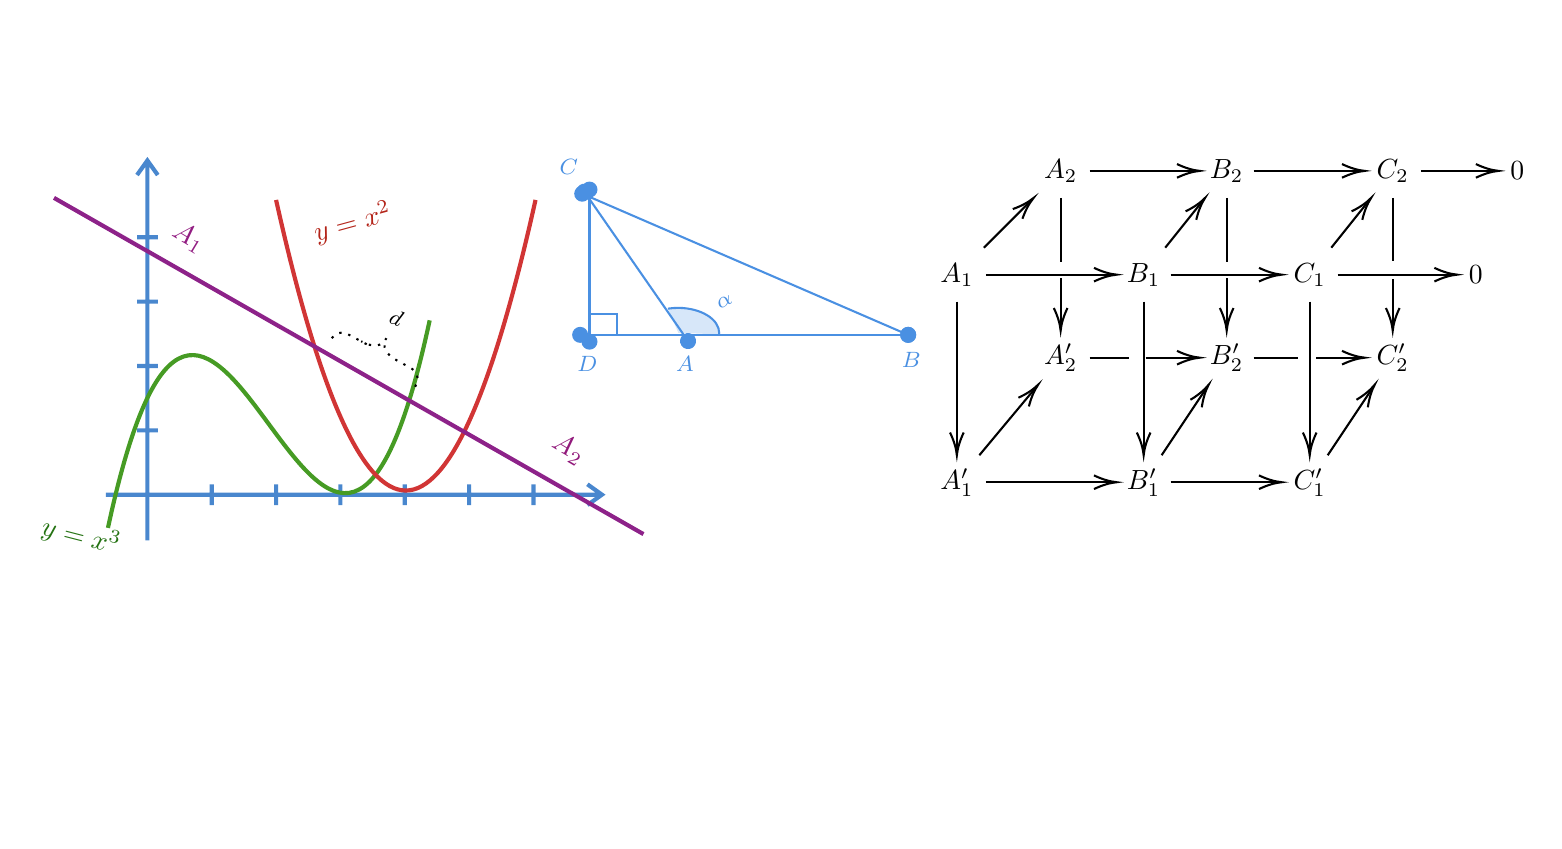
\begin{tikzpicture}[x=0.75pt,y=0.75pt,yscale=-1,xscale=1]
%uncomment if require: \path (0,235); %set diagram left start at 0, and has height of 235

%Straight Lines [id:da9313950171592851] 
\draw [color={rgb, 255:red, 74; green, 144; blue, 226 }  ,draw opacity=1 ]   (274,30) -- (274,103.29) ;
\draw [shift={(274,103.29)}, rotate = 90] [color={rgb, 255:red, 74; green, 144; blue, 226 }  ,draw opacity=1 ][fill={rgb, 255:red, 74; green, 144; blue, 226 }  ,fill opacity=1 ][line width=0.75]      (0, 0) circle [x radius= 3.35, y radius= 3.35]   ;
\draw [shift={(274,30)}, rotate = 90] [color={rgb, 255:red, 74; green, 144; blue, 226 }  ,draw opacity=1 ][fill={rgb, 255:red, 74; green, 144; blue, 226 }  ,fill opacity=1 ][line width=0.75]      (0, 0) circle [x radius= 3.35, y radius= 3.35]   ;
%Straight Lines [id:da0072983473385641595] 
\draw [color={rgb, 255:red, 74; green, 144; blue, 226 }  ,draw opacity=1 ]   (427.58,100) -- (269.5,100) ;
\draw [shift={(269.5,100)}, rotate = 180] [color={rgb, 255:red, 74; green, 144; blue, 226 }  ,draw opacity=1 ][fill={rgb, 255:red, 74; green, 144; blue, 226 }  ,fill opacity=1 ][line width=0.75]      (0, 0) circle [x radius= 3.35, y radius= 3.35]   ;
\draw [shift={(427.58,100)}, rotate = 180] [color={rgb, 255:red, 74; green, 144; blue, 226 }  ,draw opacity=1 ][fill={rgb, 255:red, 74; green, 144; blue, 226 }  ,fill opacity=1 ][line width=0.75]      (0, 0) circle [x radius= 3.35, y radius= 3.35]   ;
%Straight Lines [id:da0611422079179329] 
\draw [color={rgb, 255:red, 74; green, 144; blue, 226 }  ,draw opacity=1 ]   (270.5,32) -- (427.5,100) ;
\draw [shift={(427.5,100)}, rotate = 23.42] [color={rgb, 255:red, 74; green, 144; blue, 226 }  ,draw opacity=1 ][fill={rgb, 255:red, 74; green, 144; blue, 226 }  ,fill opacity=1 ][line width=0.75]      (0, 0) circle [x radius= 3.35, y radius= 3.35]   ;
\draw [shift={(270.5,32)}, rotate = 23.42] [color={rgb, 255:red, 74; green, 144; blue, 226 }  ,draw opacity=1 ][fill={rgb, 255:red, 74; green, 144; blue, 226 }  ,fill opacity=1 ][line width=0.75]      (0, 0) circle [x radius= 3.35, y radius= 3.35]   ;
%Straight Lines [id:da6902289836929021] 
\draw [color={rgb, 255:red, 74; green, 144; blue, 226 }  ,draw opacity=1 ]   (271.5,31) -- (321.5,103) ;
\draw [shift={(321.5,103)}, rotate = 55.22] [color={rgb, 255:red, 74; green, 144; blue, 226 }  ,draw opacity=1 ][fill={rgb, 255:red, 74; green, 144; blue, 226 }  ,fill opacity=1 ][line width=0.75]      (0, 0) circle [x radius= 3.35, y radius= 3.35]   ;
\draw [shift={(271.5,31)}, rotate = 55.22] [color={rgb, 255:red, 74; green, 144; blue, 226 }  ,draw opacity=1 ][fill={rgb, 255:red, 74; green, 144; blue, 226 }  ,fill opacity=1 ][line width=0.75]      (0, 0) circle [x radius= 3.35, y radius= 3.35]   ;
%Shape: Arc [id:dp012460516914444497] 
\draw  [draw opacity=0][fill={rgb, 255:red, 74; green, 144; blue, 226 }  ,fill opacity=0.22 ] (311.81,87.37) .. controls (313.42,87.12) and (315.12,86.99) .. (316.87,87) .. controls (327.75,87.07) and (336.54,92.5) .. (336.5,99.12) .. controls (336.5,99.34) and (336.49,99.56) .. (336.47,99.78) -- (316.8,99) -- cycle ; \draw  [color={rgb, 255:red, 74; green, 144; blue, 226 }  ,draw opacity=1 ] (311.81,87.37) .. controls (313.42,87.12) and (315.12,86.99) .. (316.87,87) .. controls (327.75,87.07) and (336.54,92.5) .. (336.5,99.12) .. controls (336.5,99.34) and (336.49,99.56) .. (336.47,99.78) ;
%Straight Lines [id:da012774030553635018] 
\draw [color={rgb, 255:red, 74; green, 144; blue, 226 }  ,draw opacity=1 ]   (274,90) -- (287.04,90) -- (287.04,100.78) ;
%Shape: Axis 2D [id:dp048941842347560494] 
\draw [color={rgb, 255:red, 73; green, 135; blue, 206 }  ,draw opacity=1 ][line width=1.5]  (41,177) -- (280,177)(61,16) -- (61,199) (273,172) -- (280,177) -- (273,182) (56,23) -- (61,16) -- (66,23) (92,172) -- (92,182)(123,172) -- (123,182)(154,172) -- (154,182)(185,172) -- (185,182)(216,172) -- (216,182)(247,172) -- (247,182)(56,146) -- (66,146)(56,115) -- (66,115)(56,84) -- (66,84)(56,53) -- (66,53) ;
\draw   ;
%Shape: Polynomial [id:dp29246577559714826] 
\draw  [color={rgb, 255:red, 70; green, 155; blue, 36 }  ,draw opacity=1 ][line width=1.5]  (42,193) .. controls (93.67,-47) and (145.33,333) .. (197,93) ;
%Shape: Parabola [id:dp636758281566334] 
\draw  [color={rgb, 255:red, 209; green, 53; blue, 53 }  ,draw opacity=1 ][line width=1.5]  (123,35) .. controls (164.67,221.67) and (206.33,221.67) .. (248,35) ;
%Straight Lines [id:da5751643928734858] 
\draw [color={rgb, 255:red, 141; green, 34; blue, 137 }  ,draw opacity=1 ][line width=1.5]    (16,34) -- (300,196) ;
%Shape: Brace [id:dp8862990797251067] 
\draw  [dash pattern={on 0.84pt off 2.51pt}] (190,125) .. controls (192.21,120.89) and (191.25,117.73) .. (187.14,115.52) -- (181.62,112.56) .. controls (175.75,109.41) and (173.91,105.77) .. (176.12,101.66) .. controls (173.91,105.77) and (169.87,106.25) .. (164,103.1)(166.64,104.52) -- (158.48,100.14) .. controls (154.37,97.93) and (151.21,98.89) .. (149,103) ;

% Text Node
\draw (339,84) node  [font=\footnotesize,color={rgb, 255:red, 74; green, 144; blue, 226 }  ,opacity=1 ,rotate=-333.43]  {$\alpha $};
% Text Node
\draw (264,19) node  [font=\footnotesize,color={rgb, 255:red, 74; green, 144; blue, 226 }  ,opacity=1 ]  {$C$};
% Text Node
\draw (273,114) node  [font=\footnotesize,color={rgb, 255:red, 74; green, 144; blue, 226 }  ,opacity=1 ]  {$D$};
% Text Node
\draw (320,114) node  [font=\footnotesize,color={rgb, 255:red, 74; green, 144; blue, 226 }  ,opacity=1 ]  {$A$};
% Text Node
\draw (429,112) node  [font=\footnotesize,color={rgb, 255:red, 74; green, 144; blue, 226 }  ,opacity=1 ]  {$B$};
% Text Node
\draw (451,71) node    {$A_{1}$};
% Text Node
\draw (501,21) node    {$A_{2}$};
% Text Node
\draw (451,171) node    {$A'_{1}$};
% Text Node
\draw (581,21) node    {$B_{2}$};
% Text Node
\draw (661,21) node    {$C_{2}$};
% Text Node
\draw (541,71) node    {$B_{1}$};
% Text Node
\draw (621,71) node    {$C_{1}$};
% Text Node
\draw (501,111) node    {$A'_{2}$};
% Text Node
\draw (581,111) node    {$B'_{2}$};
% Text Node
\draw (661,111) node    {$C'_{2}$};
% Text Node
\draw (541,171) node    {$B'_{1}$};
% Text Node
\draw (621,171) node    {$C'_{1}$};
% Text Node
\draw (721,21) node    {$0$};
% Text Node
\draw (701,71) node    {$0$};
% Text Node
\draw (81,53) node  [color={rgb, 255:red, 146; green, 29; blue, 130 }  ,opacity=1 ,rotate=-30.96]  {$A_{1}$};
% Text Node
\draw (264,155) node  [color={rgb, 255:red, 145; green, 25; blue, 123 }  ,opacity=1 ,rotate=-30.96]  {$A_{2}$};
% Text Node
\draw (29,197) node  [color={rgb, 255:red, 36; green, 114; blue, 18 }  ,opacity=1 ,rotate=-14.47]  {$y=x^{3}$};
% Text Node
\draw (160,46) node  [color={rgb, 255:red, 179; green, 35; blue, 24 }  ,opacity=1 ,rotate=-344.74]  {$y=x^{2}$};
% Text Node
\draw (181,92) node  [font=\footnotesize,rotate=-22.93]  {$d$};
% Connection
\draw    (515,21) -- (566,21) ;
\draw [shift={(568,21)}, rotate = 180] [color={rgb, 255:red, 0; green, 0; blue, 0 }  ][line width=0.75]    (10.93,-3.29) .. controls (6.95,-1.4) and (3.31,-0.3) .. (0,0) .. controls (3.31,0.3) and (6.95,1.4) .. (10.93,3.29)   ;
% Connection
\draw    (594,21) -- (645.5,21) ;
\draw [shift={(647.5,21)}, rotate = 180] [color={rgb, 255:red, 0; green, 0; blue, 0 }  ][line width=0.75]    (10.93,-3.29) .. controls (6.95,-1.4) and (3.31,-0.3) .. (0,0) .. controls (3.31,0.3) and (6.95,1.4) .. (10.93,3.29)   ;
% Connection
\draw    (464,58) -- (486.59,35.41) ;
\draw [shift={(488,34)}, rotate = 495] [color={rgb, 255:red, 0; green, 0; blue, 0 }  ][line width=0.75]    (10.93,-3.29) .. controls (6.95,-1.4) and (3.31,-0.3) .. (0,0) .. controls (3.31,0.3) and (6.95,1.4) .. (10.93,3.29)   ;
% Connection
\draw    (465,71) -- (526,71) ;
\draw [shift={(528,71)}, rotate = 180] [color={rgb, 255:red, 0; green, 0; blue, 0 }  ][line width=0.75]    (10.93,-3.29) .. controls (6.95,-1.4) and (3.31,-0.3) .. (0,0) .. controls (3.31,0.3) and (6.95,1.4) .. (10.93,3.29)   ;
% Connection
\draw    (554,71) -- (605.5,71) ;
\draw [shift={(607.5,71)}, rotate = 180] [color={rgb, 255:red, 0; green, 0; blue, 0 }  ][line width=0.75]    (10.93,-3.29) .. controls (6.95,-1.4) and (3.31,-0.3) .. (0,0) .. controls (3.31,0.3) and (6.95,1.4) .. (10.93,3.29)   ;
% Connection
\draw    (551.4,58) -- (569.35,35.56) ;
\draw [shift={(570.6,34)}, rotate = 488.66] [color={rgb, 255:red, 0; green, 0; blue, 0 }  ][line width=0.75]    (10.93,-3.29) .. controls (6.95,-1.4) and (3.31,-0.3) .. (0,0) .. controls (3.31,0.3) and (6.95,1.4) .. (10.93,3.29)   ;
% Connection
\draw    (631.4,58) -- (649.35,35.56) ;
\draw [shift={(650.6,34)}, rotate = 488.66] [color={rgb, 255:red, 0; green, 0; blue, 0 }  ][line width=0.75]    (10.93,-3.29) .. controls (6.95,-1.4) and (3.31,-0.3) .. (0,0) .. controls (3.31,0.3) and (6.95,1.4) .. (10.93,3.29)   ;
% Connection
\draw    (451,84) -- (451,156) ;
\draw [shift={(451,158)}, rotate = 270] [color={rgb, 255:red, 0; green, 0; blue, 0 }  ][line width=0.75]    (10.93,-3.29) .. controls (6.95,-1.4) and (3.31,-0.3) .. (0,0) .. controls (3.31,0.3) and (6.95,1.4) .. (10.93,3.29)   ;
% Connection
\draw    (465,171) -- (526,171) ;
\draw [shift={(528,171)}, rotate = 180] [color={rgb, 255:red, 0; green, 0; blue, 0 }  ][line width=0.75]    (10.93,-3.29) .. controls (6.95,-1.4) and (3.31,-0.3) .. (0,0) .. controls (3.31,0.3) and (6.95,1.4) .. (10.93,3.29)   ;
% Connection
\draw    (554,171) -- (605.5,171) ;
\draw [shift={(607.5,171)}, rotate = 180] [color={rgb, 255:red, 0; green, 0; blue, 0 }  ][line width=0.75]    (10.93,-3.29) .. controls (6.95,-1.4) and (3.31,-0.3) .. (0,0) .. controls (3.31,0.3) and (6.95,1.4) .. (10.93,3.29)   ;
% Connection
\draw    (629.67,158) -- (651.22,125.66) ;
\draw [shift={(652.33,124)}, rotate = 483.69] [color={rgb, 255:red, 0; green, 0; blue, 0 }  ][line width=0.75]    (10.93,-3.29) .. controls (6.95,-1.4) and (3.31,-0.3) .. (0,0) .. controls (3.31,0.3) and (6.95,1.4) .. (10.93,3.29)   ;
% Connection
\draw    (549.67,158) -- (571.22,125.66) ;
\draw [shift={(572.33,124)}, rotate = 483.69] [color={rgb, 255:red, 0; green, 0; blue, 0 }  ][line width=0.75]    (10.93,-3.29) .. controls (6.95,-1.4) and (3.31,-0.3) .. (0,0) .. controls (3.31,0.3) and (6.95,1.4) .. (10.93,3.29)   ;
% Connection
\draw    (461.83,158) -- (488.89,125.54) ;
\draw [shift={(490.17,124)}, rotate = 489.81] [color={rgb, 255:red, 0; green, 0; blue, 0 }  ][line width=0.75]    (10.93,-3.29) .. controls (6.95,-1.4) and (3.31,-0.3) .. (0,0) .. controls (3.31,0.3) and (6.95,1.4) .. (10.93,3.29)   ;
% Connection
\draw    (515,111) -- (533.95,111)(541.95,111) -- (566,111) ;
\draw [shift={(568,111)}, rotate = 180] [color={rgb, 255:red, 0; green, 0; blue, 0 }  ][line width=0.75]    (10.93,-3.29) .. controls (6.95,-1.4) and (3.31,-0.3) .. (0,0) .. controls (3.31,0.3) and (6.95,1.4) .. (10.93,3.29)   ;
% Connection
\draw    (594,111) -- (615.25,111)(624.25,111) -- (645.5,111) ;
\draw [shift={(647.5,111)}, rotate = 180] [color={rgb, 255:red, 0; green, 0; blue, 0 }  ][line width=0.75]    (10.93,-3.29) .. controls (6.95,-1.4) and (3.31,-0.3) .. (0,0) .. controls (3.31,0.3) and (6.95,1.4) .. (10.93,3.29)   ;
% Connection
\draw    (501,34) -- (501,64.72)(501,72.72) -- (501,96) ;
\draw [shift={(501,98)}, rotate = 270] [color={rgb, 255:red, 0; green, 0; blue, 0 }  ][line width=0.75]    (10.93,-3.29) .. controls (6.95,-1.4) and (3.31,-0.3) .. (0,0) .. controls (3.31,0.3) and (6.95,1.4) .. (10.93,3.29)   ;
% Connection
\draw    (581,34) -- (581,64.72)(581,72.72) -- (581,96) ;
\draw [shift={(581,98)}, rotate = 270] [color={rgb, 255:red, 0; green, 0; blue, 0 }  ][line width=0.75]    (10.93,-3.29) .. controls (6.95,-1.4) and (3.31,-0.3) .. (0,0) .. controls (3.31,0.3) and (6.95,1.4) .. (10.93,3.29)   ;
% Connection
\draw    (661,34) -- (661,64.22)(661,73.22) -- (661,96) ;
\draw [shift={(661,98)}, rotate = 270] [color={rgb, 255:red, 0; green, 0; blue, 0 }  ][line width=0.75]    (10.93,-3.29) .. controls (6.95,-1.4) and (3.31,-0.3) .. (0,0) .. controls (3.31,0.3) and (6.95,1.4) .. (10.93,3.29)   ;
% Connection
\draw    (541,84) -- (541,156) ;
\draw [shift={(541,158)}, rotate = 270] [color={rgb, 255:red, 0; green, 0; blue, 0 }  ][line width=0.75]    (10.93,-3.29) .. controls (6.95,-1.4) and (3.31,-0.3) .. (0,0) .. controls (3.31,0.3) and (6.95,1.4) .. (10.93,3.29)   ;
% Connection
\draw    (621,84) -- (621,156) ;
\draw [shift={(621,158)}, rotate = 270] [color={rgb, 255:red, 0; green, 0; blue, 0 }  ][line width=0.75]    (10.93,-3.29) .. controls (6.95,-1.4) and (3.31,-0.3) .. (0,0) .. controls (3.31,0.3) and (6.95,1.4) .. (10.93,3.29)   ;
% Connection
\draw    (674.5,21) -- (710,21) ;
\draw [shift={(712,21)}, rotate = 180] [color={rgb, 255:red, 0; green, 0; blue, 0 }  ][line width=0.75]    (10.93,-3.29) .. controls (6.95,-1.4) and (3.31,-0.3) .. (0,0) .. controls (3.31,0.3) and (6.95,1.4) .. (10.93,3.29)   ;
% Connection
\draw    (634.5,71) -- (690,71) ;
\draw [shift={(692,71)}, rotate = 180] [color={rgb, 255:red, 0; green, 0; blue, 0 }  ][line width=0.75]    (10.93,-3.29) .. controls (6.95,-1.4) and (3.31,-0.3) .. (0,0) .. controls (3.31,0.3) and (6.95,1.4) .. (10.93,3.29)   ;

\end{tikzpicture}